%%---------------------------------------------------------------------------%%
%% draco-4_0_0.tex
%% Thomas M. Evans
%% $Id$
%%---------------------------------------------------------------------------%%
\documentclass[11pt]{nmemo}
\usepackage[centertags]{amsmath}
\usepackage{amssymb,amsthm,graphicx}
\usepackage[mathcal]{euscript}
\usepackage{tmadd,tmath}
\usepackage{cite}
\usepackage{tabularx}
\usepackage{c++}

%%---------------------------------------------------------------------------%%
%% DEFINE SPECIFIC ENVIRONMENTS HERE
%%---------------------------------------------------------------------------%%
%\newcommand{\elfit}{\ensuremath{\operatorname{Im}(-1/\epsilon(\vq,\omega)}}
%\msection{}-->section commands
%\tradem{}  -->add TM subscript to entry
%\ucatm{}   -->add trademark footnote about entry

\newcommand{\draco}{Draco}
\newcommand{\dracor}{\draco-4\_0\_0}

\newcommand{\autoconf}{\textsf{Autoconf}}
\newcommand{\automake}{\textsf{Automake}} 
\newcommand{\CVS}{\textsf{CVS}}  
\newcommand{\make}{\textsf{Make}}

%%---------------------------------------------------------------------------%%
%% BEGIN DOCUMENT
%%---------------------------------------------------------------------------%%
\begin{document}

%%---------------------------------------------------------------------------%%
%% OPTIONS FOR NOTE
%%---------------------------------------------------------------------------%%

\toms{Distribution}
%\toms{Joe Sixpak/XTM, MS B226}
\refno{CCS--4:03-34(U)}
\subject{Release of \dracor}

%-------NO CHANGES
\divisionname{Computer and Computational Sciences Division}
\groupname{CCS-4:Transport Methods Group}
\fromms{Thomas M. Evans/CCS-4 D409}
\phone{(505)665--3677}
\originator{tme}
\typist{tme}
\date{9/4/2003}
%-------NO CHANGES

%-------OPTIONS
%\reference{NPB Star Reimbursable Project}
%\thru{P. D. Soran, XTM, MS B226}
%\enc{list}      
%\attachments{list}
%\cy{list}
%\encas
%\attachmentas
%\attachmentsas 
%-------OPTIONS

%%---------------------------------------------------------------------------%%
%% DISTRIBUTION LIST
%%---------------------------------------------------------------------------%%

\distribution {
  CCS--4, MS D409\\
  CCS--2, MS D413\\
}

%%---------------------------------------------------------------------------%%
%% BEGIN NOTE
%%---------------------------------------------------------------------------%%

\opening

\begin{abstract}
  We have released \dracor.  This release contains significant
  additions to the \textsc{imc} and \text{mc} packages.  Minor changes
  have been made to the \textsc{cdi} package, tools, and build system.  
\end{abstract}

%%---------------------------------------------------------------------------%%

\section{\draco\ Contributors}

The following people are contributors to \draco:
\begin{center}
  \begin{tabular}{ll}
    Tom Evans & \texttt{tme@lanl.gov} \\
    Kelly Thompson & \texttt{kellyt@lanl.gov} \\
    Todd Urbatsch & \texttt{tmonster@lanl.gov} \\
    Kent Budge & \texttt{kgbudge@lanl.gov} \\
    Mike Buksas & \texttt{mwbuksas@lanl.gov} \\
    Jim Warsa & \texttt{warsa@lanl.gov} \\
    Rob Lowrie & \texttt{lowrie@lanl.gov} \\
    Todd Adams & \texttt{bta@lanl.gov} \\
    Paul Batcho & \texttt{batcho@lanl.gov} \\
  \end{tabular}
\end{center}

%%---------------------------------------------------------------------------%%

\section{\draco\ Component Packages}

\dracor\ contains the following component packages:
\begin{center}
  \begin{tabularx}{\linewidth}{
      >{\setlength{\hsize}{.5\hsize}}L %
      >{\setlength{\hsize}{1.5\hsize}}X}    
    \hline\hline 

    c4 & communication library \\
    cdi & Common Data Interface (CDI) component \\
    cdi\_analytic & CDI analytic data component \\
    cdi\_eospac & CDI EOSPAC wrapper \\
    cdi\_gandolf & CDI GANDOLF wrapper \\
    ds++ & data structures library \\
    imc & Implicit Monte Carlo physics component \\ 
    lapack\_wrap & wrapper to BLAS and LAPACK \\
    mc & Monte Carlo physics component \\
    meshReaders & mesh reader interface \\
    meshReaders\_Services & services for mesh readers (connectivity,
    etc) \\ 
    pcgWrap & wrapper for PCGLIB \\
    plot2D & 2-D plotter interface built on XMGRACE \\
    quadrature & quadrature component \\
    rng & random number generators and SPRNG wrappers \\
    RTT\_Format\_Reader & \texttt{meshReaders} implementation for RTT
    format meshes \\
    stdheaders & C-standard libraries wrapped in the \texttt{std::}
    namespace \\ 
    timestep & a timestep controller component \\
    traits & traits used by other \draco\ components \\
    units & a physics units component \\
    viz & interfaces to visualization tools (EnSight)\\
    xm & glommable expression templates \\  

    \hline\hline 
  \end{tabularx}
\end{center}
The following table summarizes changes to \draco\ components since
\draco-3\_2\_0. 
\begin{center}
  \begin{tabularx}{\linewidth}{
      >{\setlength{\hsize}{.5\hsize}}L %
      >{\setlength{\hsize}{1.5\hsize}}X}    
    \hline\hline 

    mc & finished surface definitions \\
    imc & random walk improvements, random walk and surface tracking
    available for all particle types, new objects builder based on
    Factory Pattern \\
    cdi & optimizations to Planckian integrators
    Draco Build System & optimization flags for \textsf{gcc} updated
    \\
    tools & added features to texttt{package\_depends.py} tool \\

    \hline\hline 
  \end{tabularx}
\end{center}

There are no inter/intra-component cyclic dependencies in \draco.  The
levelized graph for \dracor\ components is shown in
Fig.~\ref{fig:level}.
\begin{figure}
  \label{fig:level}
  \centerline{
    \includegraphics[height=5.5in]{level-3_0_0.ps}}
  \caption{\dracor\ levelized component graph.  Dotted lines signify
    that the dependency if only required for testing.}
\end{figure}

Lines-of-Code (LOC) statistics for the component packages in \dracor\ 
are shown in Fig.~\ref{fig:stats}.  The aggregate LOC statistics for
\dracor\ are:
\begin{center}
  \begin{tabular}{|l|l|} \hline
    Total component package source code & 17892 \\
    Total unit test code & 21884 \\
    Total DBC statements & 2138 \\
    Total comments & 39229 \\
    \hline
  \end{tabular}
\end{center}
\begin{figure}
  \label{fig:stats}
  \centerline{
    \includegraphics[width=6in]{loc-3_2_0.eps}}
  \caption{LOC statistics for \dracor\ component packages.}
\end{figure}

LOC metrics are stored in \draco\ in \texttt{draco/doc/code\_stats}.

%%---------------------------------------------------------------------------%%

\section{Notes}

There were major build system changes between \draco-3\_1\_0 and
\draco-3\_2\_0 \cite{draco-3_2_0}.  These changes have caused some
consternation to \draco\ Build System clients.  In retrospect,
\draco-3\_2\_0 probably should have been a major release (although it
was documented like a major release in Ref. ~\ncite{draco-3_2_0}).

%%---------------------------------------------------------------------------%%

\nocite{rn98046}
\nocite{xtm:9936}
\nocite{draco-3_0_0}
\nocite{draco-4_0_0}
\bibliographystyle{rnote}
\bibliography{../bib/draco}

\closing
\end{document}

%%---------------------------------------------------------------------------%%
%% end of draco-4_0_0.tex
%%---------------------------------------------------------------------------%%
